% chap2.tex (Definitions)

\chapter{Text Classification with Deep Neural Networks}\label{TXT-CLASS}

\section{Word Embeddings}
Word embeddings are representations of words as vectors.
Neural language models, language models learned using a neural network, learn to represent words as continuous, dense vectors.
Because of the of the underlying algorithm used to learn these word embeddings, similar words tend to lie closer to each other on embedding space.
Thus, word embeddings are said to capture semantic relations, and thus encode more information than just a word identifier e.g.
a bag-of-words or one-hot vector representation.

\begin{figure}[h]
\caption{Visualization of embeddings using T-SNE. Words with similar or related meanings
tend to lie close to each other in embedding space.}
\centering
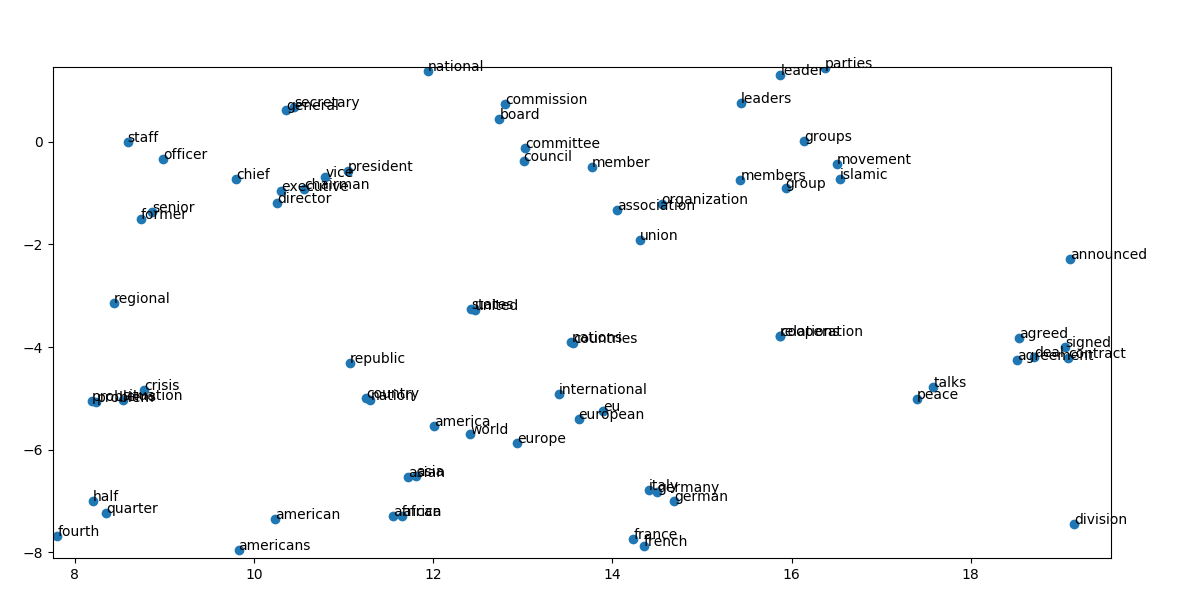
\includegraphics[width=0.5\textwidth]{EmbeddingViz.png}
\end{figure}

\section{Convolutional Neural Networks}
Convolutional neural networks are known for their abilities to learn high-level features from raw data. As input signals advance
forward through the network, they produce latent signals as linear conbinations with learned parameters, have non-linearities applied
to them, and have a pooling or selection mechanism based on simple functions such as the average or maximum operations [CITE ZHOU AND CHELLAPA 1988].

When dealing with image data, images are convolved with multiple filters, each convolution applied to overlapping subimages called as receptive fields.
This localized convolution process leads to discovery of low level features of images in the training set such as edges. As data
flows forward through the model, higher level features are discovered e.g. wheels or headlights in a vehicle image dataset.

These convolutional neural networks are comprised of \textit{feature maps}. A feature map is a \textbf{convolution} layer paired with a
\textbf{pooling} layer afterwards. The convolution stage creates \textit{activations}, whereas the pooling stage
reduces dimensionality and creates translation invariance.

\begin{figure}[H]
\caption{Visualization of a feature map with a single kernel. In this example, the kernel convolves tri-grams, or windows of three words.
After convolution with all possible trigram context windows, max pooling is applied to reduce dimensionality.
Here, the pool size is 3. This process is repeated for as many filters in the layer e.g. 100 and their outputs are
concatenated horizantally to yield a matrix of size \textit{num filters} $\times$ (\textit{input length - pool size + 1}).}
\centering
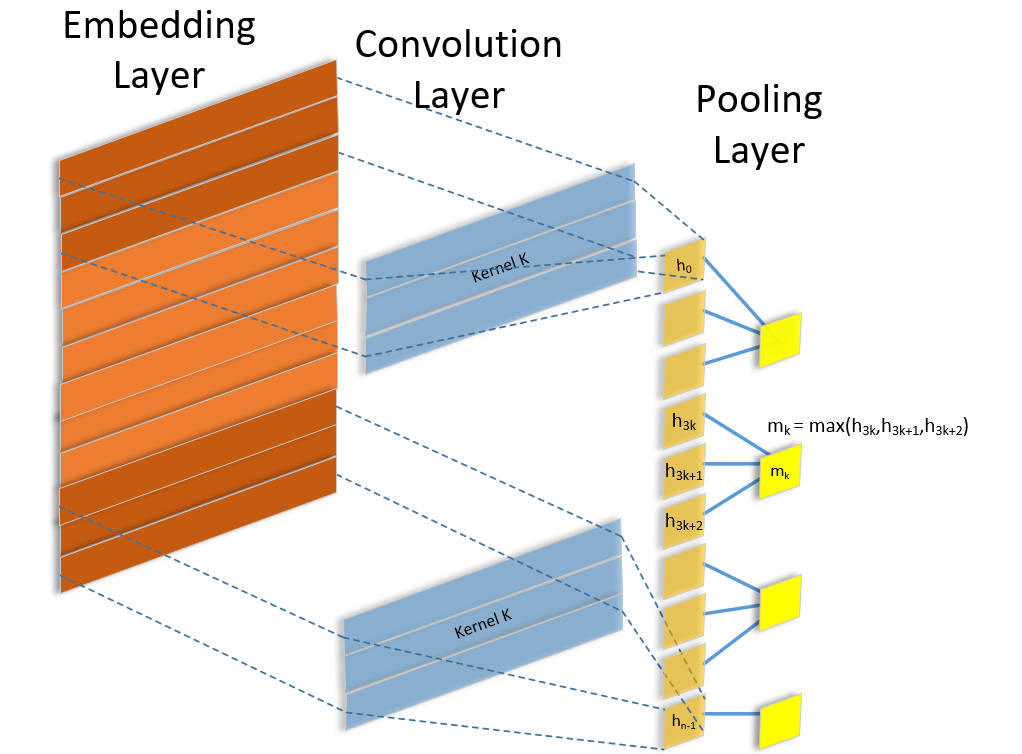
\includegraphics[width=0.5\textwidth]{FeatureMap.png}
\end{figure}

We can take advantage of word embeddings to apply convolutions to text in a fashion similar to convolutions with
image data. We apply the convolutions to overlapping sub-regions of the input text i.e. bi-grams, tri-grams, etc.
After convolving these individual and overlapping subregions, we apply a non-linear function such as $max(0,x)$ and reduce data dimensionality
by pooling.


\section{Input Representation: Integer Sequences to Word Embeddings}
Given a set of texts $\bm{s_1},...,\bm{s_m}$, we build a vocabulary $\mathbb{V}$ and a bag-of-words model from $\mathbb{V}$ to create a mapping $BoW:\mathbb{V} \mapsto \{1,...,|\mathbb{V}|\}$.
We represent a training text $\bm{s_i}$ as a sequence of integers $BoW(\bm{s})=$ $\bm{x} = x_1,...,x_k$, each integer being simply a word index
in $\mathbb{V}$. When received as input to a convolutional network, each word index will then be mapped to a corresponding embedding vector.


%%% Local Variables:
%%% mode: latex
%%% TeX-master: "thesis"
%%% End:
